\section{Access Control}
\subsection{Introduction}
Access control are a set mechanisms that guarantee that user can perform certain actions to certain resources following a \textbf{policy}. The basic AC schema is the following:
\begin{figure}[h!]
    \centering
    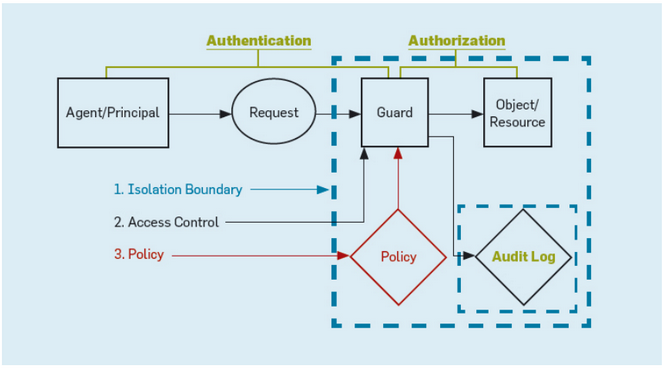
\includegraphics[scale=0.5]{images/ac.png}
    \caption{Access control schema}
    \label{fig:ac}
\end{figure}

\FloatBarrier

The agent/principal is the entity that want to access a resource, the guard is the Policy Decision Point: where the "real authorization" is computed. There is also the audit log, it allows us to perform an a posteriori reconstruction on who accessed a specific resource.

There are also two isolation boundaries:
\begin{itemize}
    \item The \textbf{outer} one prevents the by-passing of the Guard: all authorization requests go through the Guard, it can be by-passed only by privilege users.
    \item The \textbf{inner} boundary guarantees the integrity of the audit log so this can be inspected to understand what happened and why. Contrary to the other, the inner boundary cannot be by-passed even by privilege users cause that would make auditing meaningless.
\end{itemize}

An example of AC is a multiuser OS: it allows multiple user to use the same computer at the same (or different) time. This means that OS must protect users from each other (e.g. memory protection and file protection), the fundamental tradeoff of OS security is Sharing and Protection. For this purpose let's introduce the \textbf{Principle of least Priviledge:} every subject must be able to access only the information and resources that are necessary for its legitimate purpose.

So AC is the process of mediating requests to resources and data of a system and determining whether a request should be granted or denied. The flow is subject \textit{s} wants to perform action \textit{a} on a resource \textit{r}, the access request \textit{(s, a, r)} is sent to access control module that will return grant/deny. AC protect resources from unauthorized access, the security requirements are specified by \textbf{AC Policy}, a policy is a set of rules to implement specific security properties.

\myparagraph{Structured approach}
\begin{itemize}
    \item \textbf{Policy}: rules that control what actions, subjects may perform on resouces.
    \item \textbf{Model}: mathematical representation of the policy and its working.
    \item \textbf{Enforccement}: low level functions that implement the control imposed by the policy.
\end{itemize}
When policy and model are defined as mathematical objects, the meaning of policies is indipendent of a particular implementation, we apply a separation of concerns (focus on logical level and then develop the enforcement).

\subsection{AC Models}
\myparagraph{AC Matrix}
We can represent it using the Access Control Matrix, given all subjects and objects, the ACM enumerates what actions are allowed fir each subject/object pair. We create a table in which the rows are the subjects and the columns are the files, in the cell there are the actions.
\begin{table}[h!]
    \centering
    \begin{tabular}{|c|c|c|c|c|c|}
    \hline
         s/f & f1 & f2 & f3 & f4 & f5 \\
         \hline
         s1  &    & x, r, w & x & & w\\
         \hline
         s2  & x  & r, w & x, r & x & \\
         \hline
         s3  & r, w  & x, r & x, w & & r\\
         \hline
    \end{tabular}
\end{table}

\FloatBarrier

As we can see this leads us a lot of waste of space (4 blank cells), an enforcement can be use \textbf{Capabilities} and \textbf{Access Control List}.

\myparagraph{Capabilities}
In this case for each subject we have a list of file in which it has access and action that it can perform in the file.
\begin{figure}[h!]
    \centering
    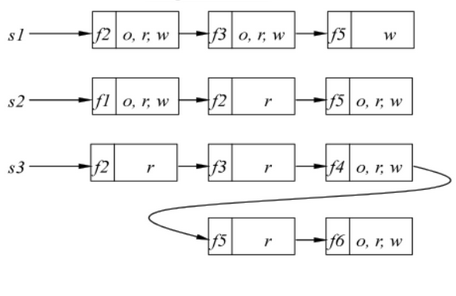
\includegraphics[scale=0.4]{images/capabilities.png}
\end{figure}

\FloatBarrier

\myparagraph{Access Control List}
In this case for each file we have a list of subjects that can access the particular file and the action that it can perform.

\begin{figure}[h!]
    \centering
    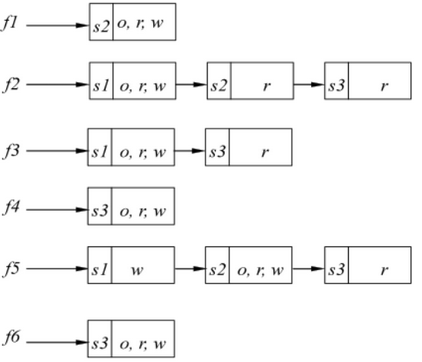
\includegraphics[scale=0.4]{images/ACL.png}
\end{figure}

\FloatBarrier

Several models exist e.g.
\begin{itemize}
    \item \textbf{DAC}: subjects can give rights to other subjects (Discretionary Access Control), it's more democratic, the owner of a resource decides how it can be shared, there isn't a central entity. It's flexible: it's easy to have multiple access to one file but it's problematic in the security point of view (Vulnerable to trojans). Usually enforced using ACL.
    \item \textbf{MAC}: system enforces mandatory rules (Mandatory Access Control). It's the opposite of DAC, one entity (king) decide for all. Usually enforced by using security labels. It's not vulnerable to trojans, it's rigid so is easy to keep the situation under control. It soffer of information leakage, still possible by covert channel.
\end{itemize}

\myparagraph{Multi-Level Security}
The goal is to define policy to prevent the release of sensitive informaitonto untrusted users, the information has different sensitivity levels and the user has different degrees of trustworthiness. Information is compartmentized into separate containers labeled according to their sensitivity label \textbf{L=(S,N)} in which S is the sensitivity and N is a set of "need-to-know" categories. Example : label (Secret, \{Nuclear, Crypto\}). At creation time, each resource is associated to a sensitivity label by resource originator according to some criteria, when a document contains both sensitive and non-sensitive information, the originator needs to use the highest appropriate level.

After associating sensitivity labels to resources, we must establish which users are authorized to access which resources, for this assign \textbf{clearances} which have the same structure of the sensitivity levels associated to resources: each user is associated to a clearance \textbf{C = (S,N)}. S is a hierarchial security level and N is a set of need-to-know categories.

We have to define two important rules:
\begin{itemize}
    \item \textit{No Read Up Property}: subject s can read resource r if it's clearance dominates the resource sensitivity label.
    \item \textit{No Write Down Property}: subject s can write to resource r if the clearance is dominated by the sensitivity label of the resource.
\end{itemize}

Implicit assumption: \textbf{Tranquillity Principle} prevents the ability to change security labels arbitrary as this can subvert security. These proprieties are at the heart of the Bell-La Padula security model introduced in 1973.
\\\\ 
If we think a lot of permissions can be grouped according to the profile of users or the set of functionalities user need to carry out their work.
\begin{figure}[h!]
    \centering
    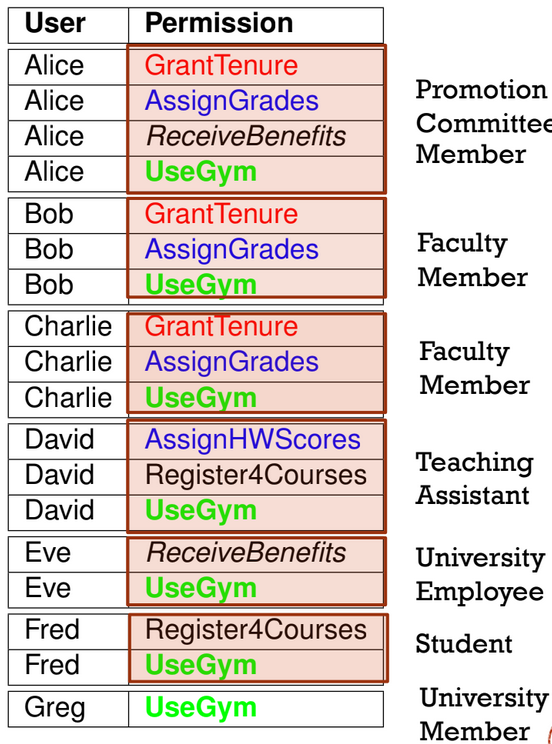
\includegraphics[scale=0.4]{images/acevolution.png}
\end{figure}
\FloatBarrier
As we see in this figure, instead of reapiting the same permissions for each user we can group them in roles, we can now split the table in two tables: one is the User Assignment (UA) table that has the User, Role binding an the other is the Permission Assignment (PA) that has the role, permission binding. Now administration is simplified, when a user gets promoted we only have to modify UA not PA. We can also do better, add a third reppresentation called Role hierarchy in which we gave an hierarchy to roles.

\subsection{Role Based Access Control}
This thing is called \textbf{RBAC}, now permission are assigned to roles rather than to individual users, users are assigned to roles rather then directky to permissions. A \textbf{role} is a job function within the context of an organization. The RBAC schema is the following:

\begin{figure}[h!]
    \centering
    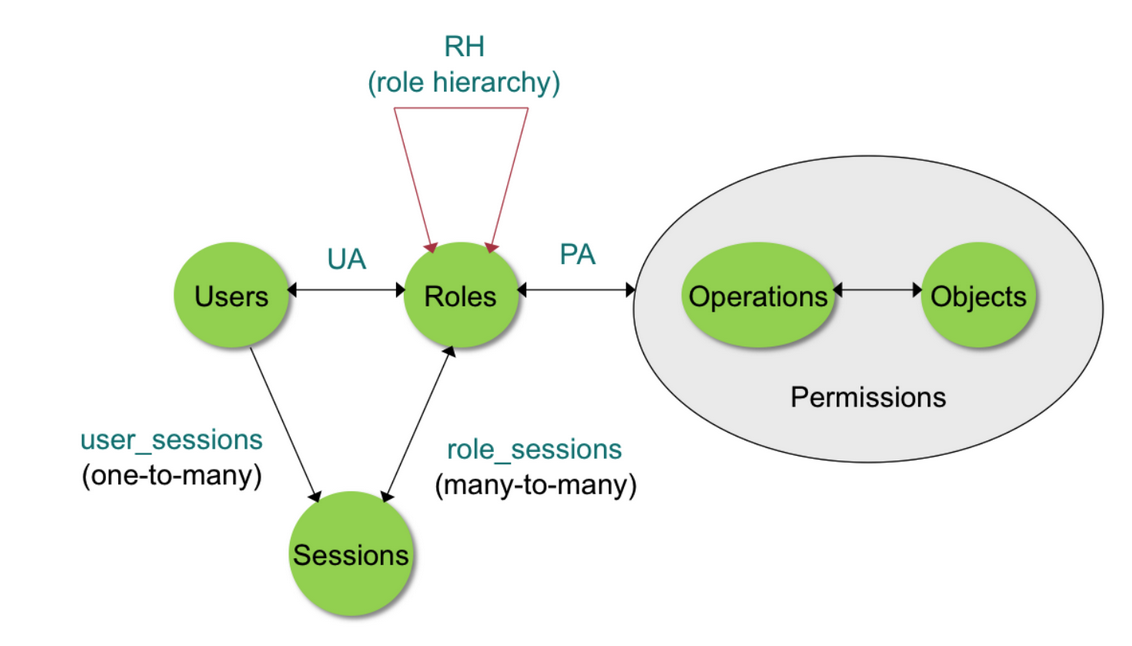
\includegraphics[scale=0.35]{images/rbac.png}
\end{figure}
\FloatBarrier
In the constrained RBAC we introduce the concept of \textbf{Separation of Duty}, is a principle that prevent user to play both role in different situation, so for example if there is a SoD for r1 and r2, u1n cannot be r1 and r2 in the same time. SoD could be static, for example the RH and UA has a static separation of duty (static because is "hardcoded"), or it could be dynamic as it is in the role\_session so for each session a user can be only r1 or r2 not both (for the single session).

\subsection{Attribute Based Access Control}
RBAC is not enaugh, roles are not the best thing for expressing authorization conditions, \textbf{ABAC} (Attribute Based Access Control) is a model that define authorizations that express conditions on properties of both the resource and the subject. It's flexible and expressive power, has the possibility to combine different patterns of authorization and consider authorization conditions depending on encironment attributes.
In ABAC the access is based on 3 different attribute types:
\begin{itemize}
    \item user attributes
    \item attributes associated with the resource to be accessed
    \item environmental conditions
\end{itemize}

\begin{figure}[h!]
    \centering
    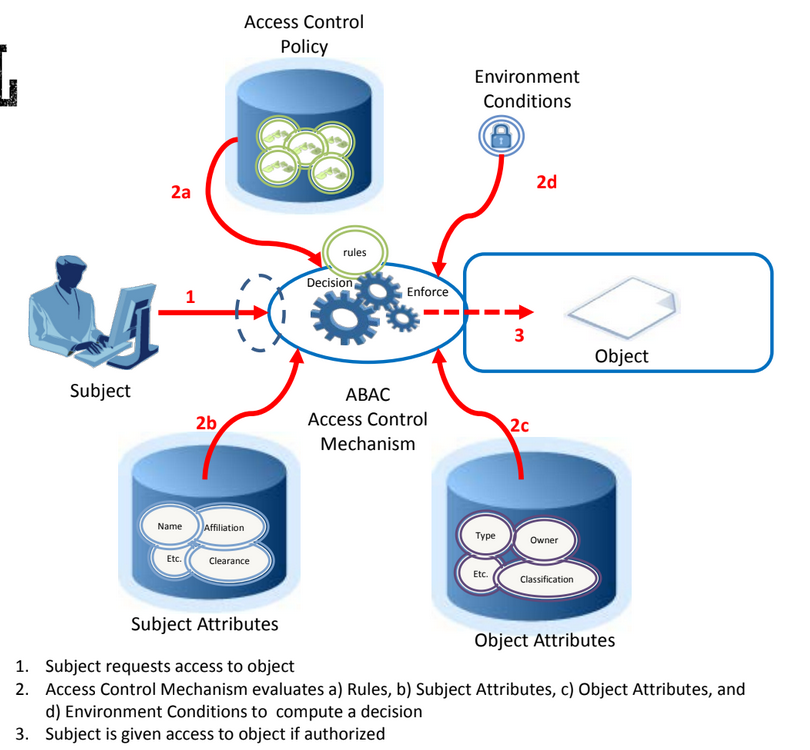
\includegraphics[scale=0.35]{images/abac.png}
\end{figure}

\FloatBarrier

In this model authorization is expressed as conditions on these attributes. ABAC has the capability to mimic previous AC models.

\subsection{XACML}
eXtensible Access Control Markup Language is an OASIS standard that was developed for collaborative environments, it can specify access control policies, access control requests and access control decisions and contains more than policy specification language. The three main components are:
\begin{itemize}
    \item XACML policy language: used for specifing access control rules.
    \item XACML request/response protocol: used to query a decision engine that evaluates user access requests against policies.
    \item XACML reference architecture
\end{itemize}
XACML \textbf{policies} are structured as PolicySets, a PolicySet consist of Policies and may include other PolicySets, Policies are composed of Rules. A target defines a Boolean condition: if True the request gets evaluated by a PDP, if False the decision is not applicable.

\begin{figure}[h!]
    \centering
    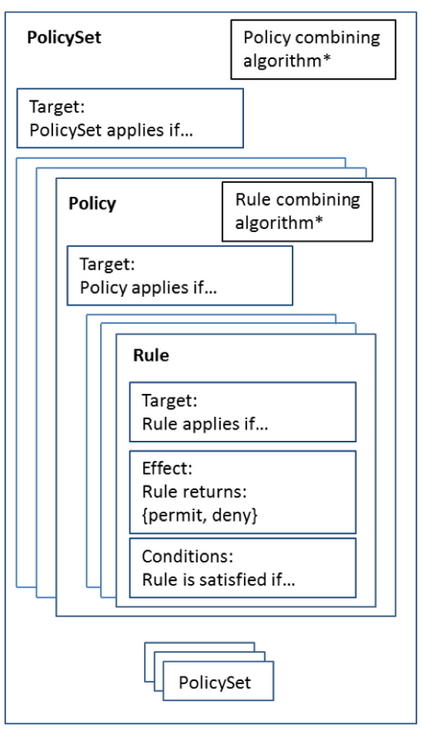
\includegraphics[scale=0.35]{images/policy.png}
\end{figure}

\FloatBarrier
XACML \textbf{rules} can evaluate to true, false or indeterminate, policies can have multiple rules and can be combined by rule combining algorithms (AND, OR, first applicable, only one applicable\footnote{if more than one decision applies, then the result is indeterminate}). XACML also include the \textbf{obligations}, this is a concept used for describing what must be carried out before or after an access request is approved and denied.
\myparagraph{XACML architecture}

\begin{figure}[h!]
    \centering
    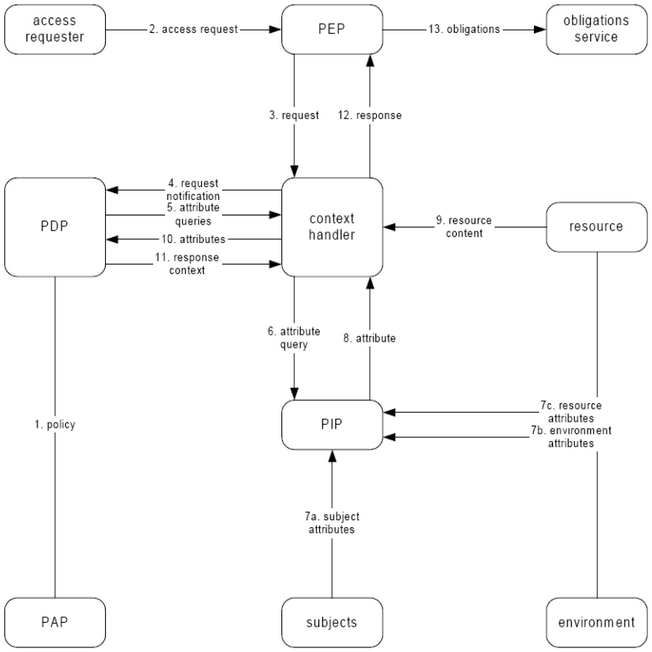
\includegraphics[scale=0.35]{images/xacml_arch.png}
\end{figure}

\FloatBarrier

\begin{itemize}
    \item \textbf{PEP}: Policy Enforcement Point, is the entity protecting the resource, performs access control by making decision requests and enforcing authorization decisions.
    \item \textbf{Context Handler}: A context is the canonical representation of a decision request and an authorization decision, it can be defined to convert the requests in its native dormat to the XACML canonical from and to convert the Authorization decisions in the XACML canonical from to the native format.
    \item \textbf{PDP}: The Policy Decision Point receives and examines the request, retrieves applicable policies, Evaluates the applicabile policy and returns the authorization decision to PEP.
    \item \textbf{PAP}: The Policy Administration Point creates security policies and stores these policies in the repository.
    \item \textbf{PIP}: The Policy Information Point serves as the source of attribute values, or the data required for policy evaluation.
\end{itemize}

\subsection{OAuth 2.0}
Let's introduce OAuth 2.0 with an example: Consider a photo lab printing your online photos, you have a lot of photos to print and you save it in a cloud folder. Straightforward implementations may request to provide your username and password to the other site but when you agree to share your secret credentials, not only do you expose your password to someone else, you also give them full access to do as they wish. This is a problem that OAuth solves, it allows users to grant access to your private resources on one site (which is the Service Provider) to another site (called Consumer/Client).

\myparagraph{How it works}
The involved entities are:
\begin{itemize}
    \item \textbf{Resource owner}: It can access to certain resources and can delegate access to resources, usually is a person.
    \item \textbf{Protected resource}: Is the service provider protecting resources for their owner, it shares resources on owner's request.
    \item \textbf{Client}: Wish to access protected resources, acts on owner's behalf.
    \item \textbf{Authorization server}: Generates tokens for the client, authenticate resource owners and clients and manages authorizations.
\end{itemize}

\begin{figure}[h!]
    \centering
    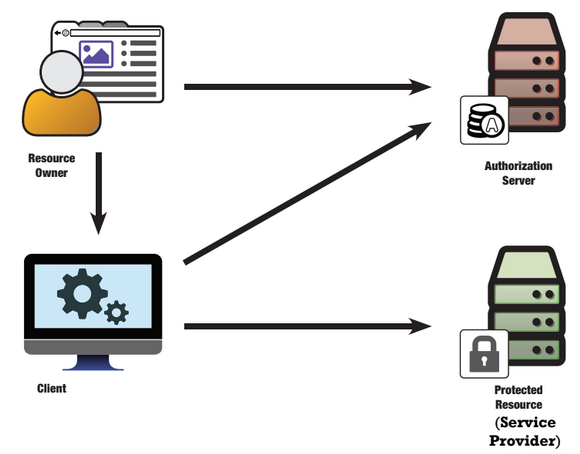
\includegraphics[scale=0.2]{images/oauth.png}
\end{figure}

\FloatBarrier

Most of the cases the Authorization server and the Service Provider live on the same server. The OAuth token is issued by authorization server and used by client, the format is opaque to client but not for AS and RS, they uderstand whats inside a token performing a database lookup, put info in the token (JWT) or RS query the AS. 

The core protocol is defined only for HTTP, it relies on TLS for securing messages. It's not an authentication protocol, authentication protocols can built using OAuth (OpenID Connect). OAuth is not a single protocol, is a framework consisting of several flows, token has not format, are opaque to the client, they need to be issued by the authorization server and understood by the resource server, but they're free to use whatever format they want (\textbf{JWT} provide a useful common format). OAuth tokens are similar to capabilities: they cam be transferred to other subjects so that permissions are delegated, permissions are decoupled from the identities of subjects.

\myparagraph{Auth Code Flow}
\begin{enumerate}
    \item Client redirects the resource owner to the authorization server's authorization endpoint.
    \item Resource owner authenticates to the authentication server.
    \item Resource owner authorizes the client.
    \item Authorization server redirects resource owner back to the client with an authorization code, this is not yet the access token that allows the client to access the protected resource.
    \item Client sends the authorization code to the authorization server's token endpoint, then client authenticates using its own credentials.
    \item Authorization server issues an OAuth access token to the client.
    \item Client accesses the protected resource using the access token.
\end{enumerate}

\myparagraph{OpenID Connect}
Authenticating resource owners to clients is out of scope for this specification, OpenID Connect defines an interoperable way to use OAuth 2.0 to perform user authentication, it is builded directly on OAuth 2.0.

\subsection{Small digression on JWT}
\textbf{JWT} (JSON Web Token) is a DeFacto standard for OAuth 2.0 access token, defines a container to transport data between interested parties, it consist of three components: the Header (identifies algorithm used to sìgn), Payload (information actually used for access control) and Signature (used to validate the token).

\begin{verbatim}
HEADER

    {
     "alg" : RS256,
     "typ" : "JWT"
    }

    baseurl64 encoded string: fseuiFAihafUIAFHsAshdf
\end{verbatim}

\begin{verbatim}
PAYLOAD

    {
     "user_name" : "admin",
    }

    baseurl64 encoded string: fseuiFAihafUIAFHsAshdf
\end{verbatim}

RS256 stays for RSA signature with SHA-256 asymmetric algorithm using a key pair, base64 is a way to encode binary data into an ASCII character set known to pretty much every computer system, base64url encoding is basically a base64 except for the use of non-reserved URL characters (e.g. \_ is used instead of /) and omit the padding characters.

The complete token is obtained by concatenating the three components above.